\documentclass[../Main.tex]{subfiles}
\begin{document}
  \chapter{2016-2017学年微积分（一）（下）期中考试}

  \section{基本计算题(每小题 6 分，共 60 分)}
  \begin{enumerate}
    \item 已知微分方程$y''+a(x)y'+b(x)y=f(x)$，$f(x)\neq0$有三个解$y_{1}=x,y_{2}
      =\mathrm{e}^{x},y_{3}=\mathrm{e}^{3x}$，求此微分方程满足初始条件$y(0)=2,y'(0)
      =3$的特解.
      \vspace{11em}

    \item 设$y=y(x)$在区间$|x|<\frac{\pi}{2}$满足微分方程$y''-(y')^{2}=1$，$y|_{x=0}
      =0$，$y'|_{x=0}=0$，求特解.
      \vspace{11em}

    \item 求过点$M(2,-2,3)$与直线$L_{1}:\frac{x+1}{1}=\frac{y-2}{2}=\frac{z-4}{0}$
      垂直相交的直线$L$的方程.
      \vspace{12em}

    \item 设曲线$\begin{cases}
        x+y-z=1,\\
        x^{2}+y^{2}+z^{2}=3
      \end{cases}$，求其在点$(1,1,1)$处的切线方程和法平面方程.
      \vspace{12em}

    \item 设$z=f(x\mathrm{e}^{y})$，其中$f$有一阶导数，$f'(0)=2$，求$\frac{\partial^{2}
      z}{\partial x\partial y}(0,1)$.
      \vspace{12em}

    \item 设函数$f(u,v,w)$有二阶连续偏导数，$z=f(x,x+y,xy)$，求混合偏导函数$\frac{\partial^{2}
      z}{\partial x\partial y}$.
      \vspace{12em}

    \item 计算$I=\int_{0}^{1}\,\mathrm{d}y\int_{y}^{\sqrt[3]{y}}\mathrm{e}^{x^{2}}\,\mathrm{d}x$.
      \vspace{12em}

    \item 计算二重积分
      \[
        I=\iint\limits_{D}\left(x^3\sin y+(x+y)^{2}\right)\,\mathrm{d}x\,\mathrm{d}y,
      \]
      其中$D:x^{2}+y^{2}\leq2y$.
      \vspace{11em}

    \item 计算三重积分$I=\iiint\limits_{V}xy^{2}z^{3}\,\mathrm{d}x\,\mathrm{d}y\,\mathrm{d}z$，其中$V$位于第一卦限，由曲面$z=0,z=xy,y=x,y=1$围成.
      \vspace{11em}

    \item 计算三重积分$I=\iiint\limits_{V}(x+z)\,\mathrm{d}v$，其中$V:\sqrt{x^{2}+y^{2}}
      \leq z\leq\sqrt{2-x^{2}-y^{2}}$.
      \vspace{11em}
  \end{enumerate}

  \section{综合计算题(每小题 8 分，共 40 分)}
  \begin{enumerate}
    \setcounter{enumi}{10}
    \item 设方程组$\begin{cases}
        F(x+y,y-z)=0,\\
        z=f(xy)
      \end{cases}$，其中$F,f$具有连续的一阶偏导，且$F_{1}-yf'F_{2}\neq0$，求$\frac{\mathrm{d}z}{\mathrm{d}y}$.
      \vspace{10em}

    \item 在椭球面$x^{2}+2y^{2}+2z^{2}=1$上求一点，使函数$f(x,y,z)=x^{2}+y^{2}
      -z$在该点处沿方向$\boldsymbol{n}=(1,-2,3)$的方向导数最大.
      \vspace{10em}

    \item 设函数$f(x)$满足$f'(x)+3f(x)+2x\int_{0}^{1}f(xt)\,\mathrm{d}t=\mathrm{e}^{-x}$，且$f(0)=1$，求$f(x)$.
      \vspace{10em}

    \item 计算$I=\iint\limits_{D}|x+y-1|\mathrm{d}x\,\mathrm{d}y$，其中$D$是圆域$D:x^{2}+y^{2}\leq1$.
      \vspace{10em}

    \item 设$f(x,y)=\sqrt[3]{x}\sqrt[3]{y^{2}}$，讨论$f(x,y)$在原点$(0,0)$处的：

      （1）连续性；

      （2）偏导数存在性；

      （3）可微性；

      （4）沿方向$\boldsymbol{n}=(\cos\alpha,\sin\alpha)$的方向导数的存在性，对存在情形计算出结果.
      \vspace{10em}
  \end{enumerate}

  \chapter{2016-2017学年微积分（一）（下）期中考试参考答案}
  \section{基本计算题(每小题 6 分，共 60 分)}
  \begin{enumerate}
    \item \textbf{Solution}. 因$\mathrm{e}^{x}-x,\mathrm{e}^{3x}-x$是齐次方程$y''
      +a(x)y'+b(x)y=0$的两个线性无关解，
      
      所以原微分方程的通解为
      \[
        y=C_{1}(\mathrm{e}^{x}-x)+C_{2}(\mathrm{e}^{3x}-x)+x.
      \]

      将$y(0)=2,y'(0)=3$代入上式，得$C_{1}=C_{2}=1$，故所求特解为
      \[
        y=\mathrm{e}^{x}+\mathrm{e}^{3x}-x.
      \]

    \item \textbf{Solution}. 令$p(x)=y'$，则原方程化为$p'=p^{2}+1,p|_{x=0}=0$.

      分离变量得
      \[
        \frac{\mathrm{d}p}{1+p^{2}}=\mathrm{d}x.
      \]

      积分得$\arctan p=x+C$，由初始条件得$C=0$，所以$p=y'(x)=\tan x$.
      再积分，并代入$y|_{x=0}=0$，得
      \[
        y(x)=-\ln(\cos x),\qquad |x|<\frac{\pi}{2}.
      \]

    \item \textbf{Solution}. 过点$M(2,-2,3)$且与直线$L_{1}$垂直的平面方程为
      \[
        (x-2)+2(y+2)=0.
      \]

      将$L_{1}$的参数方程$x=-1+t,y=2+2t,z=4$代入平面方程，得$t=-1$，从而交点为$P(-2,0,4)$.

      所求直线为过点$M$和点$P$的直线，故其方程为
      \[
        \frac{x+2}{4}=\frac{y}{-2}=\frac{z-4}{-1}.
      \]

    \item \textbf{Solution}. 令
      \[
        F(x,y,z)=x+y-z-1,\qquad G(x,y,z)=x^{2}+y^{2}+z^{2}-3.
      \]

      则
      \[
        \nabla F=(1,1,-1),\qquad \nabla G(1,1,1)=2(1,1,1).
      \]

      切线方向向量可取
      \[
        \boldsymbol{s}=(1,1,-1)\times(1,1,1)=2(1,-1,0).
      \]

      所以切线方程为
      \[
        \frac{x-1}{1}=\frac{y-1}{-1}=\frac{z-1}{0},
      \]
      法平面方程为
      \[
        x-y=0.
      \]

    \item \textbf{Solution}. 因
      \[
        \frac{\partial z}{\partial x}=\mathrm{e}^{y}f'(x\mathrm{e}^{y}),
      \]
      所以
      \[
        \frac{\partial z}{\partial x}(0,y)=\mathrm{e}^{y}f'(0)=2\mathrm{e}^{y}.
      \]

      由偏导定义可知
      \[
        \frac{\partial^{2}z}{\partial x\partial y}(0,1)
        =\left.\frac{\mathrm{d}}{\mathrm{d}y}\left(2\mathrm{e}^{y}\right)\right|_{y=1}=2\mathrm{e}.
      \]

    \item \textbf{Solution}. 记$f_{i},f_{ij}$分别为$f(u,v,w)$关于第$i$个变量的一阶偏导和二阶偏导.

      因为
      \[
        \frac{\partial z}{\partial x}=f_{1}+f_{2}+yf_{3},
      \]
      所以
      \[
        \begin{aligned}
          \frac{\partial^{2}z}{\partial x\partial y}
          &=f_{12}+xf_{13}+f_{22}+xf_{23}+f_{3}+yf_{32}+xyf_{33}\\
          &=f_{12}+xf_{13}+f_{22}+(x+y)f_{23}+f_{3}+xyf_{33}.
        \end{aligned}
      \]

    \item \textbf{Solution}. 交换积分次序，得
      \[
        I=\int_{0}^{1}\mathrm{e}^{x^{2}}\,\mathrm{d}x\int_{x^{3}}^{x}\,\mathrm{d}y
        =\int_{0}^{1}\mathrm{e}^{x^{2}}(x-x^{3})\,\mathrm{d}x.
      \]

      令$t=x^{2}$，则
      \[
        I=\frac{1}{2}\int_{0}^{1}\mathrm{e}^{t}(1-t)\,\mathrm{d}t=\frac{\mathrm{e}-2}{2}.
      \]

    \item \textbf{Solution}.

      \noindent
      \begin{minipage}[c]{0.60\textwidth}
        由于$D$关于$y$轴对称，$\iint\limits_D x^3\sin y\,\mathrm{d}x\,\mathrm{d}y=0$，
        $\iint\limits_D2xy\,\mathrm{d}x\,\mathrm{d}y=0$. 因此利用极坐标代换得
        \[
          \begin{aligned}
            I&=\iint\limits_{D}(x^{2}+y^{2})\,\mathrm{d}x\,\mathrm{d}y\\
             &=\int_{0}^{\pi}\,\mathrm{d}\theta\int_{0}^{2\sin\theta}r^{2}\cdot r\,\mathrm{d}r\\
             &=4\int_{0}^{\pi}\sin^{4}\theta\,\mathrm{d}\theta
              =8\int_{0}^{\frac{\pi}{2}}\sin^{4}\theta\,\mathrm{d}\theta
              =\frac{3\pi}{2}.
          \end{aligned}
        \]
      \end{minipage}
      \hfill
      \begin{minipage}[c]{0.30\textwidth}
        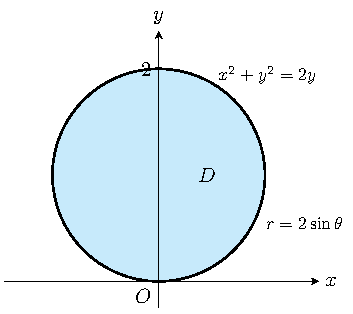
\includegraphics[width=\linewidth]{2017x-figure1.pdf}
      \end{minipage}

    \item \textbf{Solution}. 记$D$为$V$在$xOy$面上的投影，则$D$由直线$x=0,y=x,y=1$围成.
      因此
      \[
        \begin{aligned}
          I&=\iint\limits_{D}\,\mathrm{d}x\,\mathrm{d}y\int_{0}^{xy}xy^{2}z^{3}\,\mathrm{d}z\\
           &=\frac{1}{4}\iint\limits_{D}x^{5}y^{6}\,\mathrm{d}x\,\mathrm{d}y\\
           &=\frac{1}{4}\int_{0}^{1}\,\mathrm{d}x\int_{x}^{1}x^{5}y^{6}\,\mathrm{d}y\\
           &=\frac{1}{28}\int_{0}^{1}(x^{5}-x^{12})\,\mathrm{d}x
            =\frac{1}{28}\left(\frac{1}{6}-\frac{1}{13}\right) = \frac{1}{312}.
        \end{aligned}
      \]

    \item \textbf{Solution}.

      \noindent
      \begin{minipage}[c]{0.60\textwidth}
        由对称性可得$\iiint\limits_{V}x\,\mathrm{d}v=0$.

        用柱坐标代换，得
        \[
          \begin{aligned}
            I&=\iiint\limits_{V}z\,\mathrm{d}v\\
             &=\int_{0}^{2\pi}\,\mathrm{d}\theta\int_{0}^{1}r\,\mathrm{d}r
              \int_{r}^{\sqrt{2-r^{2}}}z\,\mathrm{d}z\\
             &=\pi\int_{0}^{1}(2-2r^{2})r\,\mathrm{d}r=\frac{\pi}{2}.
          \end{aligned}
        \]
      \end{minipage}
      \hfill
      \begin{minipage}[c]{0.30\textwidth}
        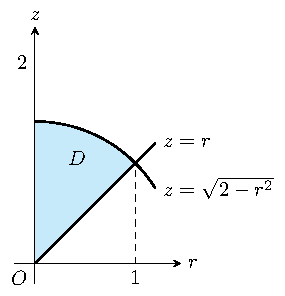
\includegraphics[width=\linewidth]{2017x-figure2.pdf}
      \end{minipage}
  \end{enumerate}

  \section{综合计算题(每小题 8 分，共 40 分)}
  \begin{enumerate}
    \setcounter{enumi}{10}
    \item \textbf{Solution}. 视$x,z$为因变量，方程组两边对$y$求导，得
      \[
        \begin{cases}
          F_{1}\left(\dfrac{\mathrm{d}x}{\mathrm{d}y}+1\right)
          +F_{2}\left(1-\dfrac{\mathrm{d}z}{\mathrm{d}y}\right)=0,\\[8pt]
          \dfrac{\mathrm{d}z}{\mathrm{d}y}=f'\left(x+y\dfrac{\mathrm{d}x}{\mathrm{d}y}\right).
        \end{cases}
      \]

      于是
      \[
        \frac{\mathrm{d}z}{\mathrm{d}y}
        =\frac{f'\left[(x-y)F_{1}-yF_{2}\right]}{F_{1}-yf'F_{2}}.
      \]

    \item \textbf{Solution}. 设所求点为$M(x,y,z)$，则$\nabla f(M)=(2x,2y,-1)$，且
      $\boldsymbol{n}^{\circ}=\frac{1}{\sqrt{14}}(1,-2,3)$.

      函数$f(x,y,z)$在点$M$处沿方向$\boldsymbol{n}$的方向导数为
      \[
        \frac{\partial f(M)}{\partial \boldsymbol{n}}
        =\frac{1}{\sqrt{14}}(2x-4y-3).
      \]

      即在约束$x^{2}+2y^{2}+2z^{2}=1$下求$2x-4y-3$的最大值. 构造Lagrange函数
      \[
        L(x,y,z,\lambda)=2x-4y-3+\lambda(x^{2}+2y^{2}+2z^{2}-1).
      \]

      令
      \[
        \begin{cases}
          L_{x}=2+2\lambda x=0,\\
          L_{y}=-4+4\lambda y=0,\\
          L_{z}=4\lambda z=0,\\
          L_{\lambda}=x^{2}+2y^{2}+2z^{2}-1=0.
        \end{cases}
      \]

      得$x=-y,z=0$. 代入约束方程，得
      \[
        x=\pm\frac{\sqrt3}{3},\qquad y=\mp\frac{\sqrt3}{3},\qquad z=0.
      \]

      比较方向导数的值，可知所求点为
      \[
        \left(\frac{\sqrt3}{3},-\frac{\sqrt3}{3},0\right).
      \]

    \item \textbf{Solution}. 令$u=tx$，则
      \[
        x\int_{0}^{1}f(tx)\,\mathrm{d}t=\int_{0}^{x}f(u)\,\mathrm{d}u.
      \]

      从而原方程变为
      \[
        f'(x)+3f(x)+2\int_{0}^{x}f(u)\,\mathrm{d}u=\mathrm{e}^{-x}.
      \]

      由上式可知$f''(x)$存在，两边求导得
      \[
        f''(x)+3f'(x)+2f(x)=-\mathrm{e}^{-x}. \tag{*}
      \]

      特征方程$r^{2}+3r+2=0$有相异实根$r=-2,-1$，对应齐次方程通解为
      \[
        Y=C_{1}\mathrm{e}^{-2x}+C_{2}\mathrm{e}^{-x}.
      \]

      设特解为$y^{*}=Ax\mathrm{e}^{-x}$，代入方程(*)得$A=-1$，所以
      \[
        f(x)=C_{1}\mathrm{e}^{-2x}+C_{2}\mathrm{e}^{-x}-x\mathrm{e}^{-x}.
      \]

      由原方程可得$f'(0)=-2$，又$f(0)=1$，代入得$C_{1}=0,C_{2}=1$.
      因此
      \[
        f(x)=(1-x)\mathrm{e}^{-x}.
      \]

    \item \textbf{Solution}.

      \noindent
      \begin{minipage}[c]{0.60\textwidth}
        用$x+y=1$将区域$D$分为
        
        $D_{1}=D\cap\{(x,y)\mid x+y\geq1\}$和$D_{2}=D\setminus D_{1}$.

        记$g=x+y-1$，则
        \[
          \begin{aligned}
            I&=\iint\limits_{D_{1}}g\,\mathrm{d}\sigma-\iint\limits_{D_{2}}g\,\mathrm{d}\sigma\\
             &=2\iint\limits_{D_{1}}g\,\mathrm{d}\sigma-\iint\limits_{D}g\,\mathrm{d}\sigma.
          \end{aligned}
        \]

        因为
        \[
          \iint\limits_{D}g\,\mathrm{d}\sigma=\iint\limits_{D}(-1)\,\mathrm{d}x\,\mathrm{d}y=-\pi,
        \]
        且
        \[
          \begin{aligned}
            \iint\limits_{D_{1}}g\,\mathrm{d}\sigma
            &=\int_{0}^{1}\,\mathrm{d}x\int_{1-x}^{\sqrt{1-x^{2}}}(x+y-1)\,\mathrm{d}y\\
            &=\frac{5}{6}-\frac{\pi}{4}.
          \end{aligned}
        \]

        所以
        \[
          I=\frac{5}{3}+\frac{\pi}{2}.
        \]
      \end{minipage}
      \hfill
      \begin{minipage}[c]{0.30\textwidth}
        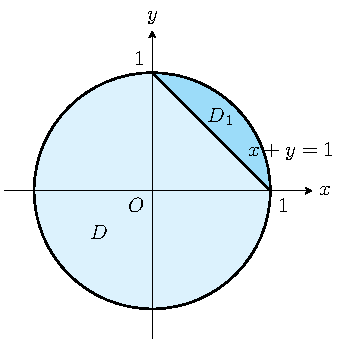
\includegraphics[width=\linewidth]{2017x-figure3.pdf}
      \end{minipage}

    \item \textbf{Solution}.

      （1）由于$f(x,y)=\sqrt[3]{x}\sqrt[3]{y^{2}}$是初等函数，且在全平面有定义，所以$f(x,y)$在$(0,0)$处连续.

      （2）因为$f(x,0)=0$，所以$f_{x}(0,0)=0$；同理$f_{y}(0,0)=0$.

      （3）考虑极限
      \[
      \begin{aligned}
          \lim_{(x,y)\to(0,0)}\frac{f(x,y)-f(0,0)-f_{x}(0,0)x-f_{y}(0,0)y}{\sqrt{x^{2}+y^{2}}} = \lim_{(x,y)\to(0,0)}\frac{\sqrt[3]{x}\sqrt[3]{y^{2}}}{\sqrt{x^{2}+y^{2}}}
      \end{aligned}
      \]
      考虑$y=x$，$(x,y)\to(0,0)$时，$\lim_{x\to0}\frac{\sqrt[3]{x}\sqrt[3]{x^{2}}}{\sqrt{2}|x|}=\frac{1}{\sqrt{2}}\lim_{x\to0}\frac{x}{|x|}$不存在，所以$f(x,y)$在$(0,0)$处不可微.

      （4）利用方向导数的定义，得
      \[
        \frac{\partial f(0,0)}{\partial \boldsymbol{n}}
        =\lim_{\rho\to0^{+}}\frac{f(\rho\cos\alpha,\rho\sin\alpha)}{\rho}
        =\sqrt[3]{\cos\alpha}\sqrt[3]{\sin^{2}\alpha}.
      \]
  \end{enumerate}
\end{document}






